\documentclass[a4paper,12pt]{article}
\usepackage[utf8]{inputenc}
\usepackage{graphicx,amsmath, amsthm, amssymb, color, wrapfig}
\usepackage{placeins}
\usepackage{fancyvrb}
\usepackage{listings}

\usepackage[round]{natbib}
\bibliographystyle{elsarticle-harv}

\lstset{
 numbers=left,
 basicstyle=\fontsize{11}{13}\selectfont\ttfamily,
 stepnumber=1,    
 firstnumber=1,
 numberfirstline=true
}

\begin{document}

\title{AnisoPedCTM Manual}
\author{Flurin H\"anseler \& Gael Lederrey \\ Transport and Mobility Laboratory, EPFL}

\date{\today}
\maketitle

% - - - - - - - - - - - - - - - - - INTRODUCTION - - - - - - - - - - - - - - - - - 
\section{Introduction}

AnisoPedCTM is a Java implementation of a macroscopic model for  time-varying, anisotropic and congested pedestrians flows. It is jointly developed by EPFL and PolyU Hong Kong \citep{heart2015}. It can be used to generate textual and/or graphical output. A framework for its calibration on walking time data using pseudo maximum likelihood is included.

\section{Program Structure}

The model is composed of different classes. 

\renewcommand\labelitemi{{\boldmath$\cdot$}}

\begin{itemize}
\item \verb+AnisoPedCTM.java+ is the main class. The user explicitly selects the scenario files for the experiment, as well as the different files for the calibration. Multiple examples are given in this file.
\item \verb+Board.java+ is where the computations are done.
\item \verb+Calibration.java+ contains the calibration process.
\end{itemize}
All the following classes represent distinct objects needed for the computation. They describe the model framework and are characterized by parameters, a constructor, and all the functions interacting with the parameters. This concerns: 
\begin{itemize}
\item \verb+Cell.java+
\item \verb+Fragment.java+
\item \verb+Group.java+
\item \verb+Link.java+
\item \verb+Node.java+
\item \verb+Pedestrian.java+
\item \verb+Route.java+
\end{itemize}
\verb+PotentialField.java+ computes the potential of nodes.\\
\newline
\verb+Parameter.java+ describes all the parameters needed to run the entire program going from the input to the output files. \\
\newline
\verb+FunDiag.java+ is an abstract class that defines the Fundamental Diagram. There are four other classes that inherit from this class. Each defines a distinct Fundamental Diagram.

\begin{itemize}
\item \verb+FunDiagDrake.java+: the Drake Fundamental Diagram.
\item \verb+FunDiagSbFD.java+: the Stream-base Fundamental Diagram (proposed model).
\item \verb+FunDiagWeidmann.java+: the Weidmann Fundamental Diagram.
\item \verb+FunDiagZero.java+: a fundamental diagram with constant speed (for benchmarking).
\end{itemize}
The \verb+Visualization.java+ class creates the graphical output.\\
\newline
The \verb+Input.java+ and \verb+Output.java+ classes deal with the inputs and the outputs.\\
 \newline
Finally, there is a \verb+Debug.java+ class to debug the program if needed.

% - - - - - - - - - - - - - - - - - HOW USE IT - - - - - - - - - - - - - - - - - 
\section{How to use it}
\subsection{Requirements}
In order to run AnisoPedCTM properly, several text (.txt) files have to be specified before running the application. Examples of these files are given in the folder examples.

% - - - - - - - - - - - - - - - - - DEMAND FILE - - - - - - - - - - - - - - - - -
\subsubsection{Demand file}
This file contains the disaggregate trip table. Each line corresponds to a pedestrian. It is characterized by a route (\verb+routeName+) where the origin and the destination nodes are specified, a departure time (\verb+departureTime+) and a travel time (\verb+travelTime+), given both in [sec]. The travel time is optional, needed only for the calibration.

Example:
\begin{lstlisting}[breaklines]
#routeName,depTime,travelTime
W->E,0,8.1925
N->E,1,9.2166
S->W,2.20,10.659
W->N,3.60,20.78
\end{lstlisting}

\subsubsection{Network folder}
This folder describes the network topology using three files:
\begin{enumerate}
\item Cells: A cell is characterized by a name (\verb+cellName+), a zone (\verb+zone+) to which the cell belongs, a surface in [m$^2$] (\verb+surfaceSize+) and 4 pair coordinates (\verb+coordinate pairs+) that represent the corners of the cell in cartesian coordinates. Note that origin-destination cells have typically an infinite surface size (\verb+INF+).

Example: 
\begin{lstlisting}[breaklines]
#cellName, zone, surfaceSize [m2], coordinate pairs of each corner
NW, ZNW, INF, (-1.5|4) (-0.5|4) (-0.5|5) (-1.5|5)
NWGATE, ZNWGATE, INF, (-1.5|3) (-0.5|3) (-0.5|4) (-1.5|4)
\end{lstlisting}

\item Links: A link is characterized by the name of the containing cell (\verb+cellName+), the name of the origin cell (\verb+origCellName+), the name of the destination cell (\verb+destCellName+), and a length (\verb+length+). The links also have a flow direction, given by the origin (\verb+streamOrig+) and the destination (\verb+streamDest+) of the stream. Finally, a boolean indicator (\verb+bi-directional+) tells if pedestrians can cross the link in both directions. (Note that in the manuscript, links are referred to as streams, whereas here a distinction between pedestrian streams and physical links are made. This is useful for the notation of the computational model, but unnecessarily complicates the mathematical model.)

Example:
\begin{lstlisting}[breaklines]
#cellName, origCellName, destCellName, length, streamOrig, streamDest, boolean bi-directional
NW, none, NWGATE, MIN, N, S, true
NWGATE, NW, A2, MIN, N, S, true
\end{lstlisting}

\item Routes: A route is characterized by a name (\verb+routeName+) and a sequence of zones (\verb+zoneSequence+) which contains all the cells where the route passes. The order in which zones appear in that sequence is irrelevant (the sequence is thus rather a set).

Example: 
\begin{lstlisting}[breaklines]
#routeName, zoneSequence
NW->SWHELPER, ZNW-ZNWGATE-ZCENTER-ZSWHELPERGATE-ZSWHELPER
N->W, ZN-ZNGATE-ZCENTER-ZWGATE-ZW
N->E, ZN-ZNGATE-ZCENTER-ZEGATE-ZE
\end{lstlisting}
\end{enumerate}

% - - - - - - - - - - - - - - - - - PARAMETERS FILE - - - - - - - - - - - - - - - - -
\subsubsection{Parameters file}
For each type of Fundamental Diagram, different parameters, which are specific to each model, are needed.
\newline\newline
Example: 

\begin{lstlisting}[breaklines]
#FunDiag: Drake
vf [m/s], 1.3085816218836281
thetaDrake [m^4], 0.13314813025718492
mu [-], 1.2964392184766242
\end{lstlisting}

\begin{itemize}
\item Line 1 defines which version of the FD is used. It is only a comment, and has no functional purpose.
\item Line 2 defines the global free-flow speed in [m/s].
\item Line 3 defines the $\vartheta$ parameter of the Drake model.
\item Line 4 defines the path choice parameter $\mu$.
\end{itemize}
Similarly we have for the others FDs: 

\begin{lstlisting}[breaklines]
#FunDiag: SbFD
vf [m/s], 1.3077965456196432
theta [m^4], 0.14327777730206429
beta [m^2], 0.3026551512486577
mu [-], 2.539811911178543
\end{lstlisting}

\begin{itemize}
\item Line 3 defines the $\vartheta$ parameter of the SbFD model.
\item Line 4 defines the $\beta$ parameter of the SbFD model. 
\end{itemize}

\begin{lstlisting}[breaklines]
#FunDiag: Weidmann
vf [m/s], 1.3353356914195833
gamma [1/m^2], 1.6619179475396773
kj [1/m^2], 5.990409148005435
mu [-], 2.036556238435761
\end{lstlisting}

\begin{itemize}
\item Line 3 defines the shape parameter $\gamma$ of the Weidmann model.
\item Line 4 defines the jam density parameter $k_\text{jam}$ of the Weidmann model. 
\end{itemize}

\begin{lstlisting}[breaklines]
#FunDiag: Zero
vf [m/s], 1.3085816218836281
mu [-], 1.2964392184766242
\end{lstlisting}
The parameter search space file specifies the search intervals for each parameter in the calibration process.
\newline\newline
Example for the Drake FD: 

\begin{lstlisting}[breaklines]
#FunDiag: Drake
vf [m/s], 0.8, 1.2
thetaDrake [m^4], 1e-5, 0.4
mu [-], 1.0, 15.0
\end{lstlisting}

% - - - - - - - - - - - - - - - - - SCENARIO FILE - - - - - - - - - - - - - - - - -
\subsubsection{Scenario file}

This is the configuration file. It contains all the information of the experiment to run. The user can enable or disable several features from this file, for instance regarding the calibration. It is composed of different sections: 

\begin{itemize}
\item Configuration file section: Contains the path directory information of the input/output folders, the file names of the content of the network folder, which Fundamental Diagram it uses and the Courant-Fiedrichs-Lewy (CFL, typically 1.0) factor.
\item Output section: The user can activate/deactivate the text or debug output.
\item Visualization section: the user can activate/deactiva the visualization output as well as the display of the cell names and the numbers. The correspondences file name needs to be given. The correspondence file is a mapping between the cardinal points (N,S,E,W) and the four directions UP, DOWN, RIGHT, and LEFT. It is used to correctly draw the arrows in the output.\\
\newline
Example of correspondence file: 

\begin{lstlisting}[breaklines]
# Give the correspondences between N, S, E, W and UP, DOWN, RIGHT, LEFT (Separation with a ',')
N, UP
S, DOWN
E, RIGHT
W, LEFT
\end{lstlisting}

\item Demand section:  The user can choose the demand format between aggregate and disaggregate. The demand file name has to be given and it can be chosen whether to write the aggregated table or not.
\item Calibration section: The parameter search range file path has to be given as well as the calibration mode and the aggregation period (in [sec]).
\end{itemize}
Example: 
\begin{small}
\begin{lstlisting}[breaklines]
#configuration file (do not change order of parameters)
input directory: examples/
output directory: examples/output/HKU-sbfd/86/
parameter file name: parameters/sbfdParamHKU.txt
link configuration file name: networks/HKU_links.txt
cell configuration file name: networks/HKU_cells.txt
route configuration file name: networks/HKU_routes.txt
fundamental diagram: SbFD
CFL factor: 1.0

# Output
text output: false
debug output: false

# Visualization
visualization: true
display cell names: false
display numbers: true
correspondences (visualization) file name: parameters/correspondences_visualization.txt

# Demand
demand format: disaggregate
demand file name: demand/HKU-86_180_86_18-68.txt
write aggregated table: false

# Calibration
parameter search range file: parameters/sbfdParamSearchSpace.txt
calibration mode: travel time distribution
aggregation period (sec): 6
\end{lstlisting}
\end{small}

% - - - - - - - - - - - - - - - - - OUTPUT - - - - - - - - - - - - - - - - - 
\subsection{Output}

All the outputs generated by AnisoPedCTM are in the \verb+output+ folder.

% - - - - - - - - - - - - - - - - - TEXT OUTPUT - - - - - - - - - - - - - - - - - 

\subsubsection{Text output}

The following text output is generated by default. The date in the file contains the day the user runs the program (in order not to accidentally overwrite previous runs). The last number corresponds to the number of iterations made during the calibration process.

\begin{itemize}
\item \verb+calibStatistics-2015-9-26_32.txt+: This file contains information about the calibration process. It gives the optimal parameters found as well as standard statistics used in a maximum likelihood setting.
\item \verb+travelTimeStatistics-2015-8-15_0.txt+:  The file contains statistics about travel times. It is composed of different sections: 
\begin{itemize}
\item Travel time per route: Each line is characterized by the name of the route (\verb+routeName+), the number of pedestrians (\verb+numPed+), as well as the observed and estimated travel time mean and standard deviation (\verb+travelTimeMeanObs (stDev)+ and \verb+travelTimeMeanSim (stDev)+).
\item Disaggregate OD table: Each line corresponds to a pedestrian. It is characterized by the departure time (\verb+depTime+), the route (\verb+routeName+), the travel time observed (\verb+travelTimeObs+), the estimated mean of the travel time (\verb+travelTimeMeanSim+) with its standard deviation (\verb+travelTimeStdDevSim+).
\item Travel time distribution for each route: For each route, the total number of observed pedestrians (\verb+totNumObs+), and the total number of estimated pedestrians  (\verb+totNumEst+) are given. The observed and estimated walking time distribution is reported, providing for each \verb+travel time interval+ the number of observed pedestrians (\verb+numPedObs+), and the corresponding estimate (\verb+fragmentSizeEst+). 
\end{itemize}
\end{itemize}

The following text output may be turned on or off by the user:

\begin{itemize}
\item \verb+systemState.txt+: This file describes the system state at any time interval. Each of its lines contains a time interval (\verb+timeInterval+), a link ID (\verb+linkID+), a cell name (\verb+cellName+), a group ID (\verb+groupID+), and the size of the group on the link (\verb+groupSizeOnLink+).

\item \verb+travelTimeDist.txt+: This file contains the travel time distribution of each group. It is characterized by the ID of the group (\verb+groupID+), the route (\verb+routeName+), the size of the group, (\verb+groupSize+), the departure time (\verb+depTime+), the travel time (\verb+travelTime+) and the size of the fragment (\verb+fragmentSize+).

\item \verb+travelTimeMean.txt+: This file contains the mean travel time of each group. It is characterized by the ID of the group (\verb+groupID+), the name of the route the group takes (\verb+routeName+), the size of the group (\verb+groupSize+), the departure time interval (\verb+departureTime+), the total travel time (\verb+weightedTravelTime+), and the relative loss (\verb+rel_loss+; ratio of departed pedestrians reaching destination; due to numerical rounding this ratio may be lower than 1, e.g.\ 0.999).
\end{itemize}

% - - - - - - - - - - - - - - - - - GRAPHICAL OUTPUT - - - - - - - - - - - - - - - - - 
\subsubsection{Graphical output}

The graphical output may be turned on or off by the user. It appears as a folder called \verb+Pictures+. It is decomposed in four other folders and made of several images, each representing a different time interval.  

\begin{itemize}
\item Accumulation: Number of pedestrians in a cell or on a link.
\item Density: Number of pedestrians per area in a cell or on a link.
\item Flow: Number of pedestrians being propagated within a time interval with respect to a cell or a link.
\item Speed: As resulting from the fundamental diagram.
\end{itemize}
Each of these folders has the same structure. They can have two subfolders: 

\begin{itemize}
\item Cell: Where the entire cell is shaded, representing cell properties (e.g.\ cell density).
\item Copy: Where arrows are shaded, representing properties of pedestrian streams (e.g.\ stream density).
\end{itemize}
The pictures computed are available scaled or unscaled. For the scaled ones, the scale is used with two colors: blue and red (blue typically referring to the free-flow state and red referring to the congested state), while for the unscaled ones, a black-and-white scale is used.

For speed, two scaled versions are available: One with respect to the free-flow speed, and another with respect to the critical speed.
\newline\newline
Example of what can be found in each folder:

\begin{figure}[h!]
    \centering
    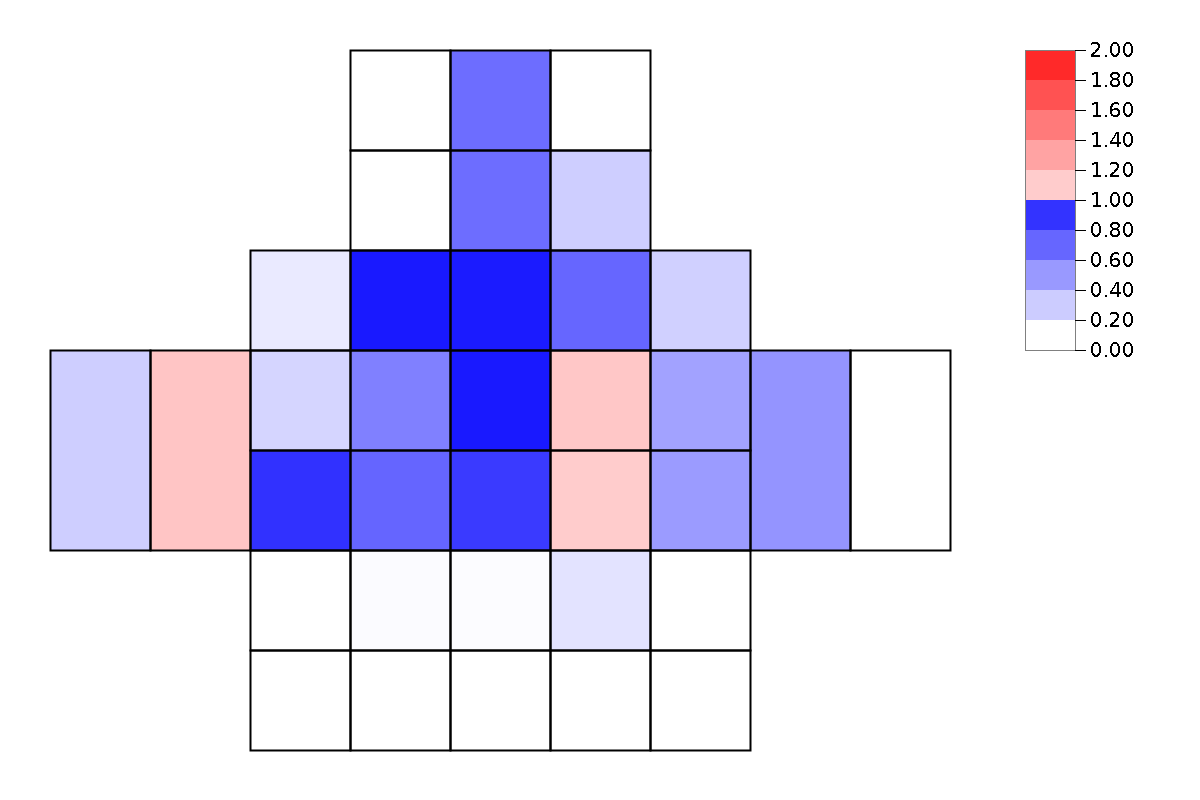
\includegraphics[width=70mm]{figures/accumulation}
    \caption{Accumulation/Cell scaled}
    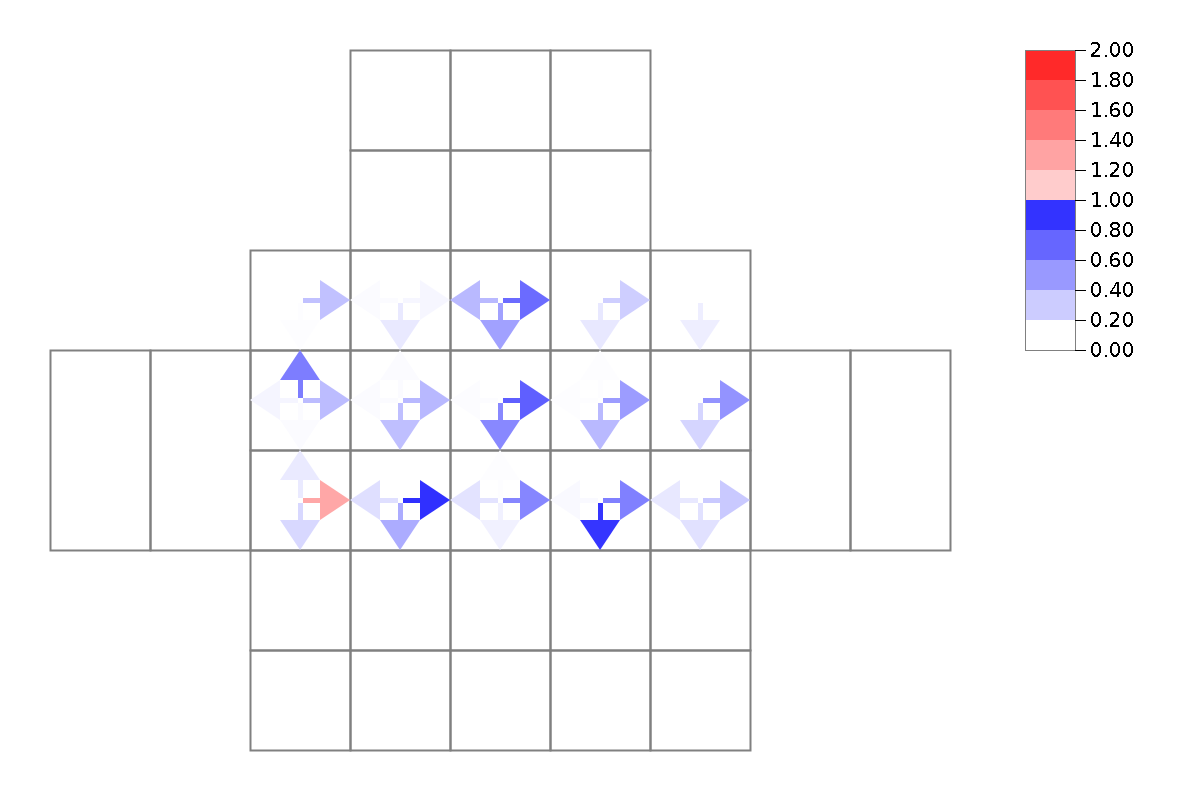
\includegraphics[width=70mm]{figures/density}
    \caption{Density/Copy scaled}
\end{figure} 
\clearpage
\begin{figure}[h!]
    \centering
    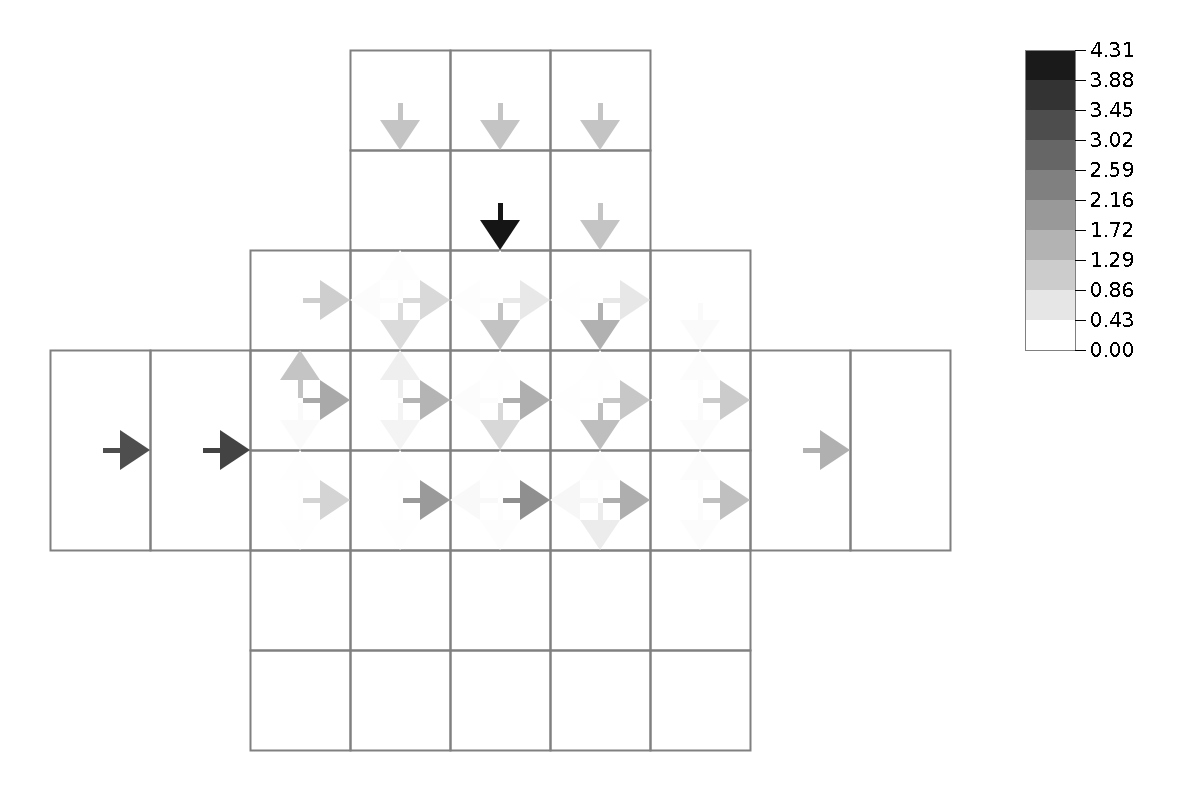
\includegraphics[width=70mm]{figures/flow}
    \caption{Flow/Copy unscaled}
\end{figure} 
\begin{figure}[h!]
    \centering
    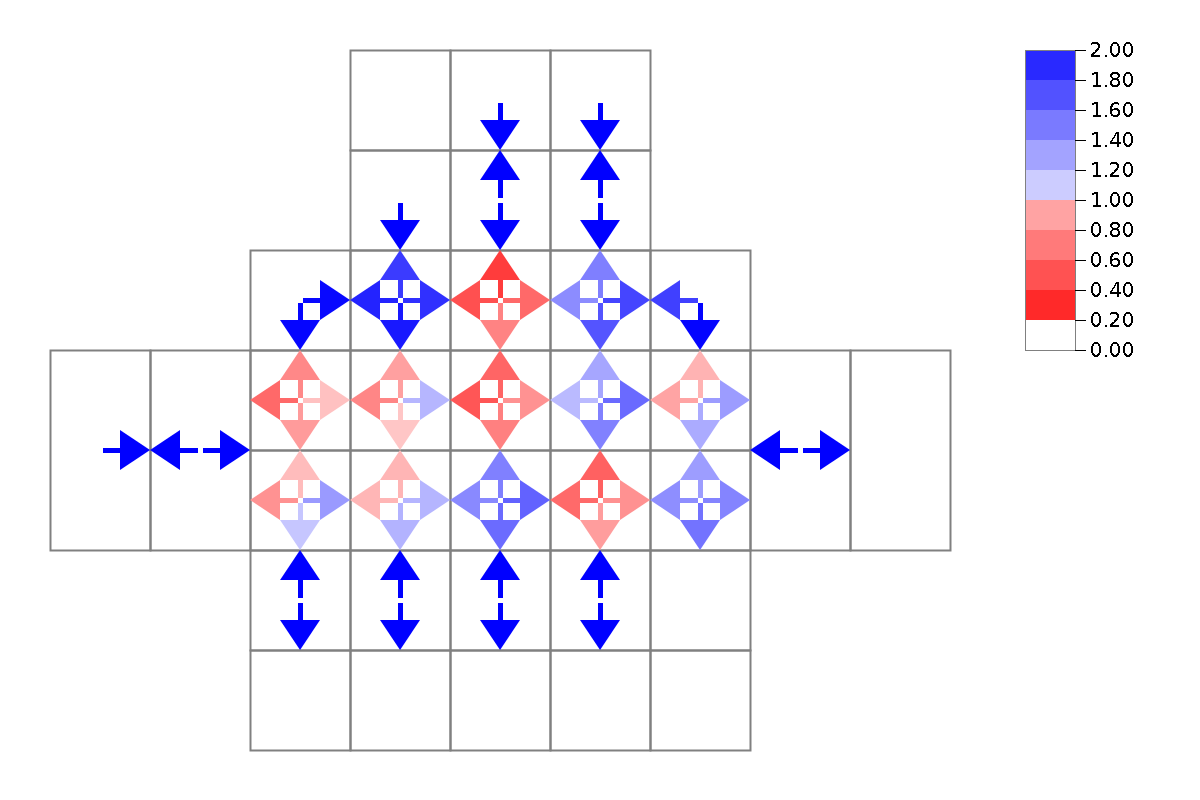
\includegraphics[width=70mm]{figures/speed}
    \caption{Speed/Copy scaled with respect to the critical speed}
\end{figure} 

\section{How to install it}

\subsection{Requirements}
Java 8 is required to run AnisoPedCTM. If no parallelization is required, Java 7 is sufficient.

\section{Acknowledgement}
This documentation has been largely written by Jo\"el Fonseca, EPFL.

\bibliographystyle{plainnat}
\bibliography{../../../../Literature/Flurin_Bibliography}

\end{document}
